\chapter{Конструкторская часть}

\section{Введение}
В данном разделе представлены схемы алгоритмов поиска подстроки в строке: стандартного алгоритма и алгоритма Бойера~---~Мура.

\section{Требования к программному обеспечению}\label{section:requirements}

Программное обеспечение должно удовлетворять следующим функциональным требованиям: на входе -- две строки, на выходе -- массив индексов исходной строки.

Программное обеспечение также должно соответствовать следующим требованиям:
\begin{itemize}[label=---]
	\item наличие пользовательского интерфейса для выбора действий;
	\item составление массива индексов вхождения подстроки в строку;
	\item предоставление функционала для измерения времени выполнения алгоритмов.
\end{itemize}

\section{Разработка алгоритмов}
В данном разделе представлены схемы алгоритмов для стандартного алгоритма поиска (рисунок \ref{img:standart}) и алгоритма Бойера~---~Мура поиска подстроки в строке (рисункок \ref{img:boyermoor}).

\begin{figure}[h]
	\centering
	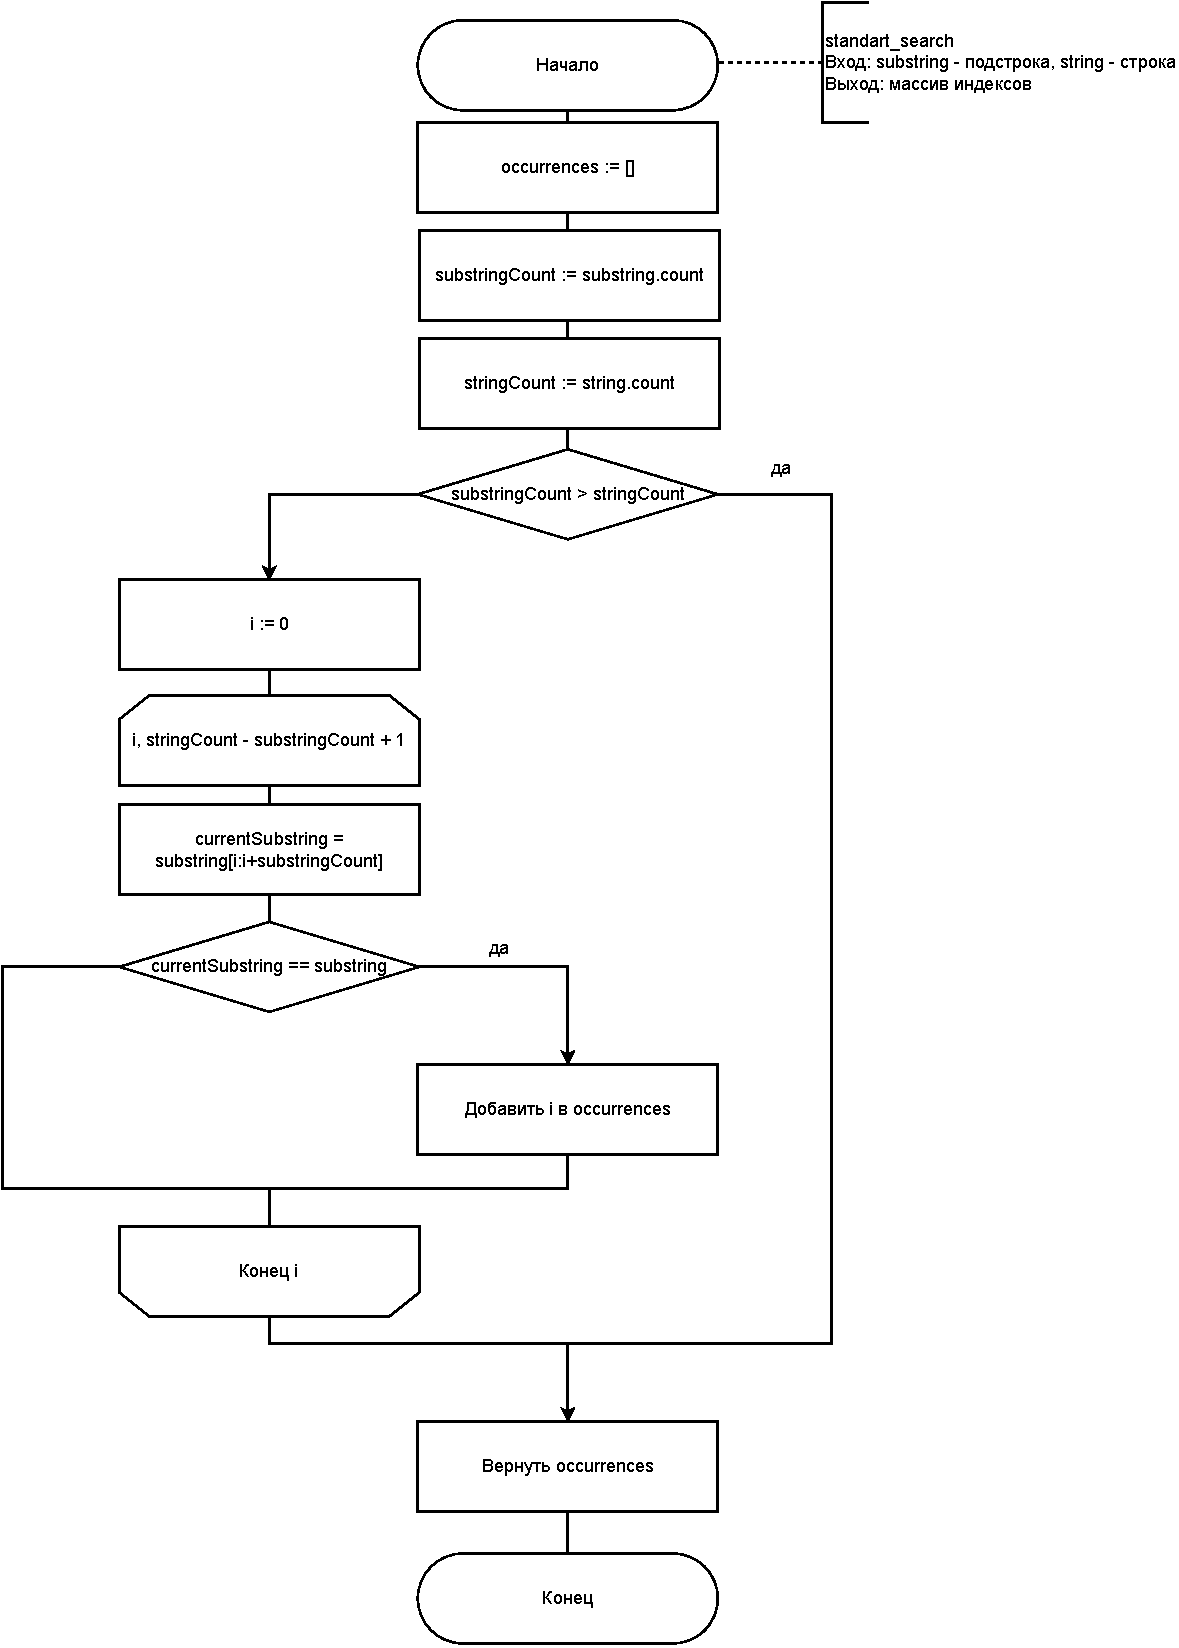
\includegraphics[width=1\linewidth]{img/standart.pdf}
	\caption{Схема стандартного алгоритма поиска подстроки в строке}
	\label{img:standart}
\end{figure}

\begin{figure}[h]
	\centering
	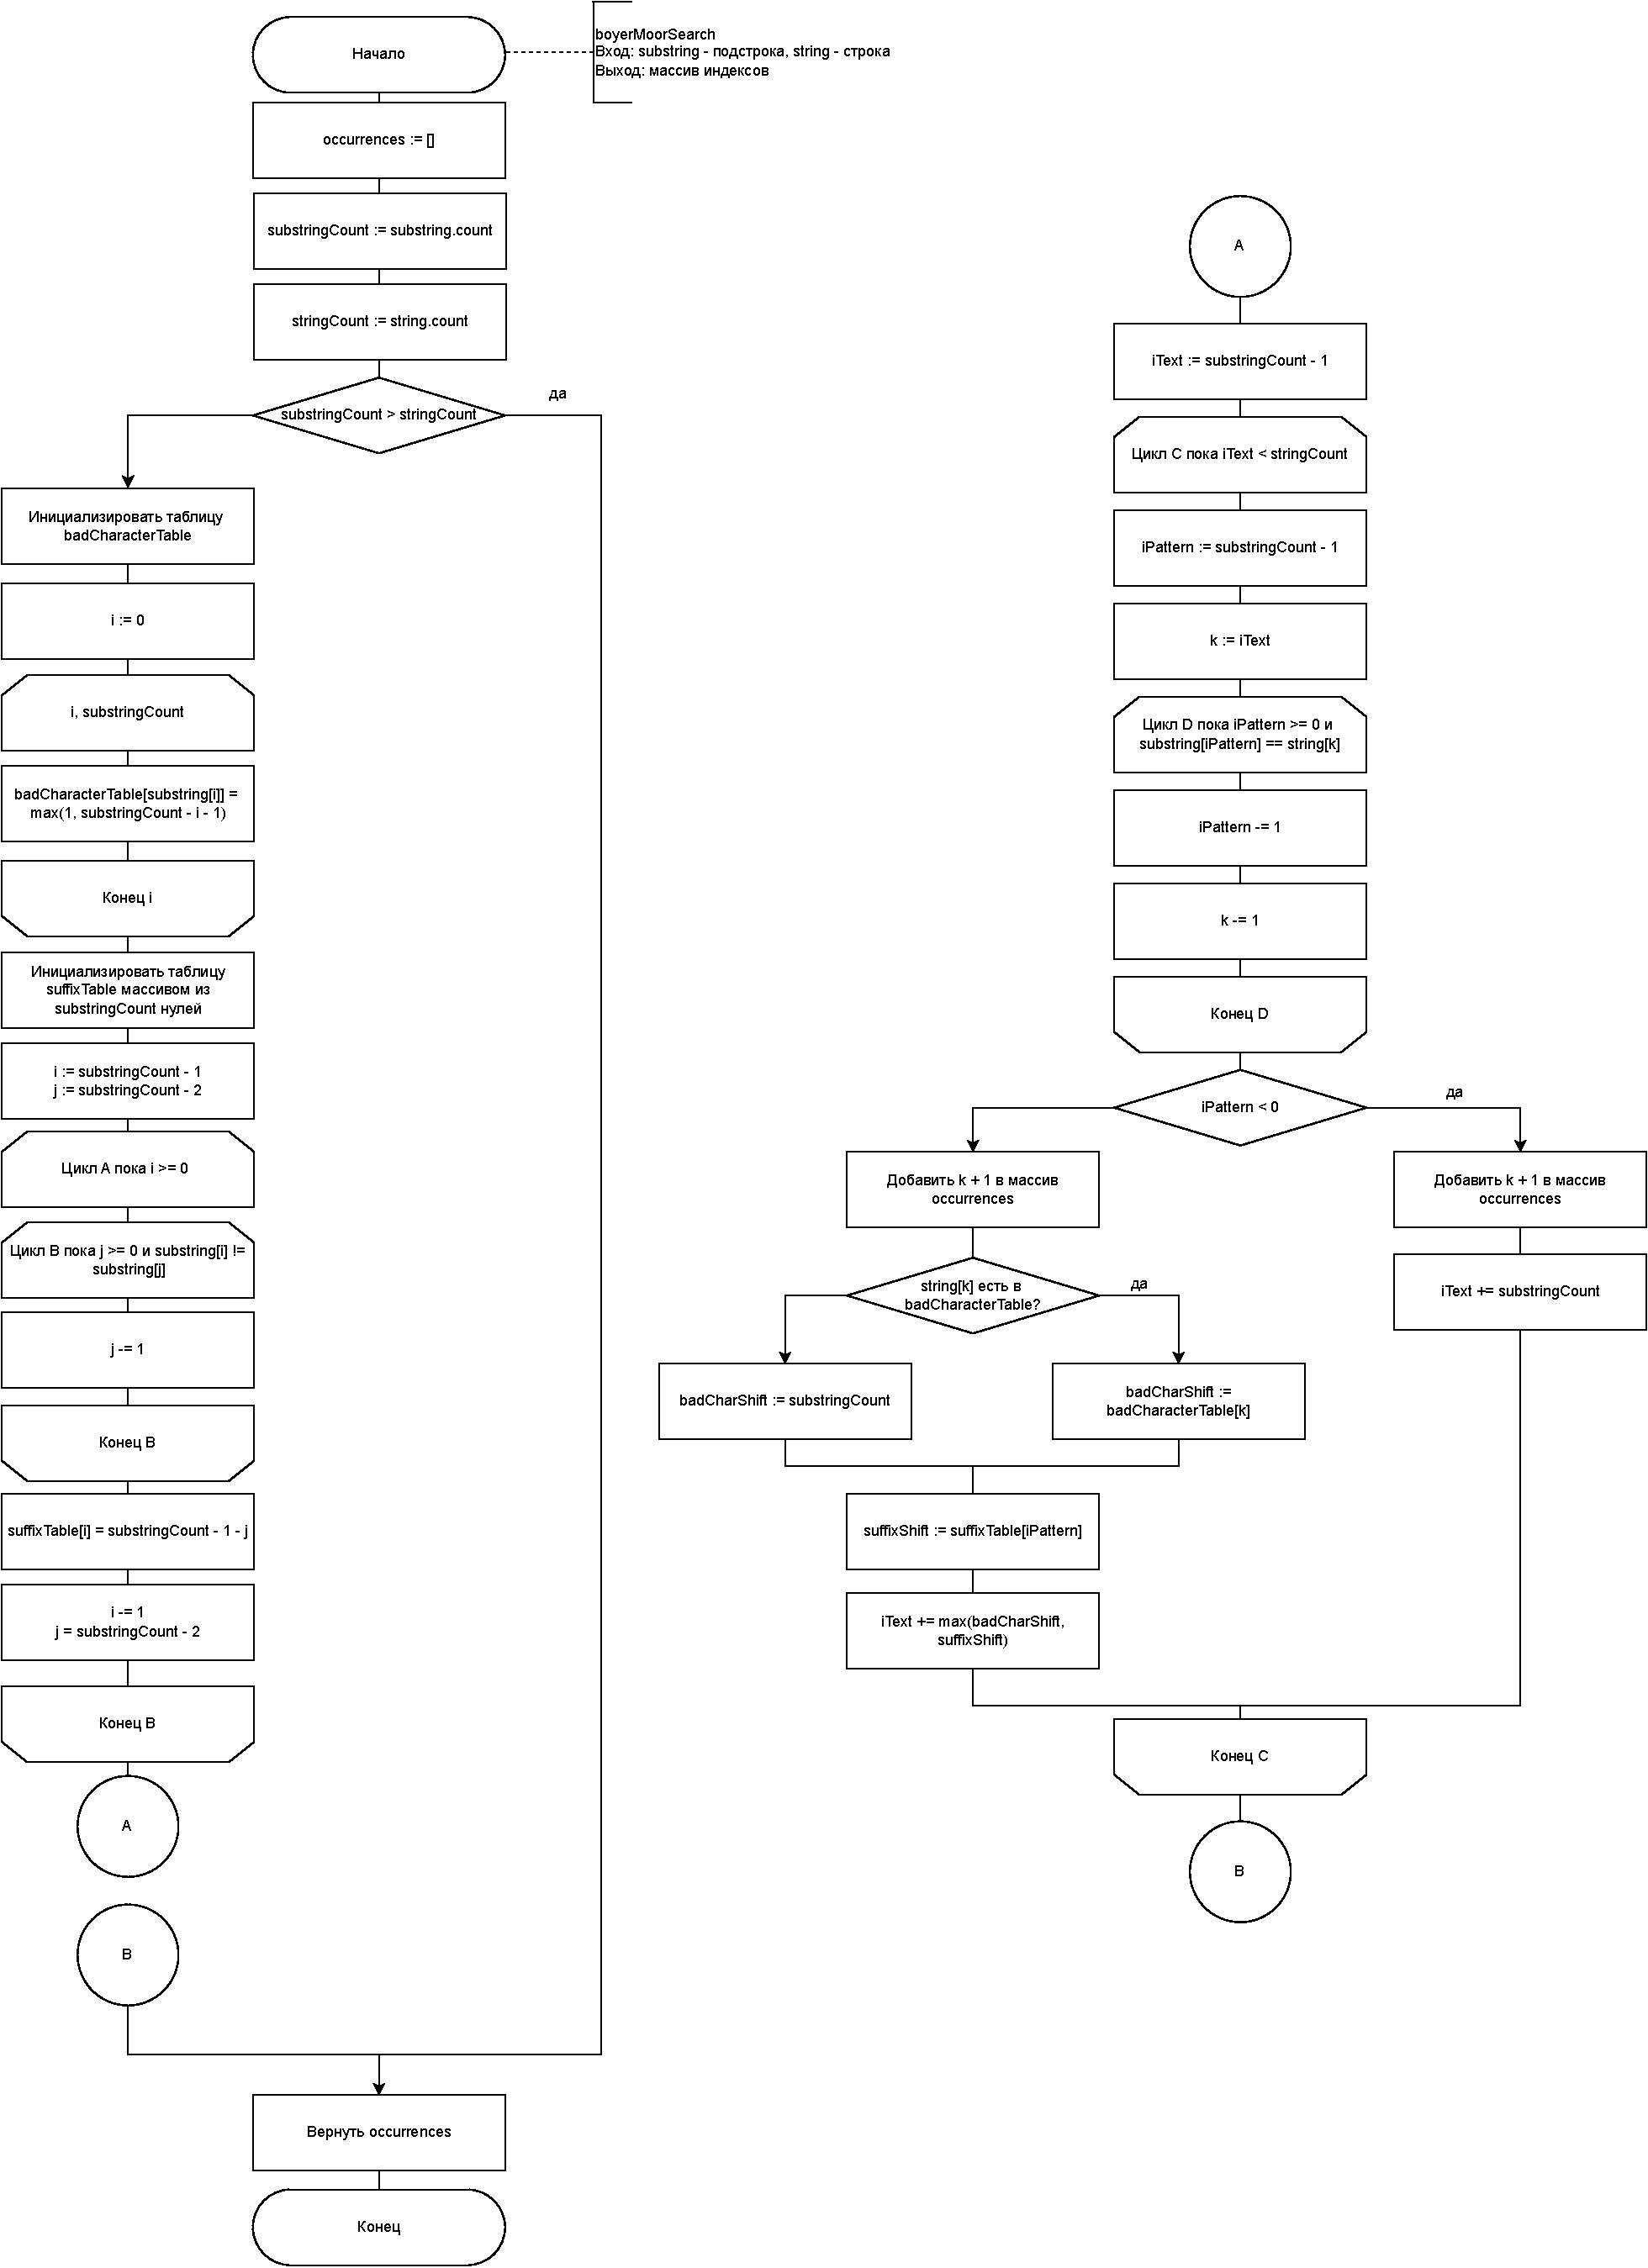
\includegraphics[width=1\linewidth]{img/boyermoor.pdf}
	\caption{Схема алгоритма Бойера~---~Мура}
	\label{img:boyermoor}
\end{figure}

\clearpage

\section*{Вывод}
В данном разделе были представлены схемы алгоритмов поиска подстроки в строке: стандартного алгоритма и алгоритма Бойера~---~Мура.
